\documentclass[a4paper,12pt]{report}
\usepackage[a4paper, portrait, margin=0.5in]{geometry}
\usepackage[utf8]{inputenc}
\usepackage{graphicx}
\usepackage{dsfont}
\usepackage{amsmath}
\usepackage{esint}
\usepackage{mathtools}
\usepackage{cancel}
\usepackage{bbold}
\usepackage{wrapfig}
\usepackage{subcaption}
\usepackage{listings}
\usepackage{xcolor}		
\usepackage{systeme}
\usepackage{soul}
\usepackage{ amssymb }

\setcounter{secnumdepth}{3}
\setcounter{tocdepth}{3}

\newcommand{\limit}[2]{\underset{#1 \rightarrow #2}{\lim} \,}
\newcommand{\arrowlim}[2]{\overset{#1 \rightarrow #2}{\longrightarrow}}
\newcommand{\arrowlimtwo}[4]{\overset{\scriptsize{\begin{array}{cc}
				#1 {}&\rightarrow #2\\
				#3 &\rightarrow #4
		\end{array}}
	}{\longrightarrow}}

\newcommand{\Lagr}{\mathcal{L}}
\newcommand{\Four}{\mathcal{F}}
\newcommand{\TdZ}{\mathcal{Z}}
\newcommand{\R}{\mathbb{R}}
\newcommand{\C}{\mathbb{C}}
\newcommand{\N}{\mathbb{N}}
\newcommand{\Z}{\mathbb{Z}}
\newcommand{\nextpassage}{\nonumber \\ &\downarrow \nonumber \\}
\newcommand{\firstpassage}{ \\ &\downarrow \nonumber \\}
\newcommand{\spacer}{\quad ; \quad}
\newcommand{\except}[1]{\backslash \{ #1 \} }
\newcommand{\taleche}{\; : \;}
\newcommand{\bolditem}[1]{\item \textbf{#1}}
\newcommand{\separator}{\nonumber \\ 
	\nonumber \\}
\newcommand{\double}[2]{\left\{ \begin{array}{cc}
		#1\\
		#2
	\end{array}
	\right.
}
\newcommand{\triple}[3]{\left\{ \begin{array}{ccc}
		#1\\
		#2\\
		#3
	\end{array}
	\right.
}	
\newcommand{\quadruple}[4]{\left\{ \begin{array}{ccc}
		#1\\
		#2\\
		#3\\
		#4
	\end{array}
	\right.
}	

\newcommand{\nosgn}{\;\;\,}

\newcommand{\quadvec}[4]{\left( \begin{array}{ccc}
		#1\\
		#2\\
		#3\\
		#4
	\end{array}
	\right)
}



%opening
\title{Simulazione di una linea di trasmissione partendo da misure parziali in laboratorio}
\author{Alessandro Marcelli}

\begin{document}

\maketitle

\begin{abstract}
Gli obiettivi originali dell'esperienza comprendevano lo studio in laboratorio delle proprietà di una linea di trasmissione, quali il coefficiente dielettrico e i fenomeni di riflessione dovuti al mancato adattamento della linea.
Causa zona rossa dovuta alla pandemia COVID è stato impossibile completare l'esperienza sulla linea di trasmissione. Partendo dai dati raccolti si è quindi simulata su SIMetrix una linea quanto più simile possibile a quella usata in laboratorio. 
\end{abstract}

\tableofcontents

\newpage
\section{Richiami di teoria}

\subsection{Linea di trasmissione infinita}
Idealmente, una linea infinita generica è un mezzo a parametri diffusi attraverso il quale viene inviato un segnale elettrico, con velocità prossima a $c$ e senza perdite. 
\begin{figure}[!htb]
	\centering
	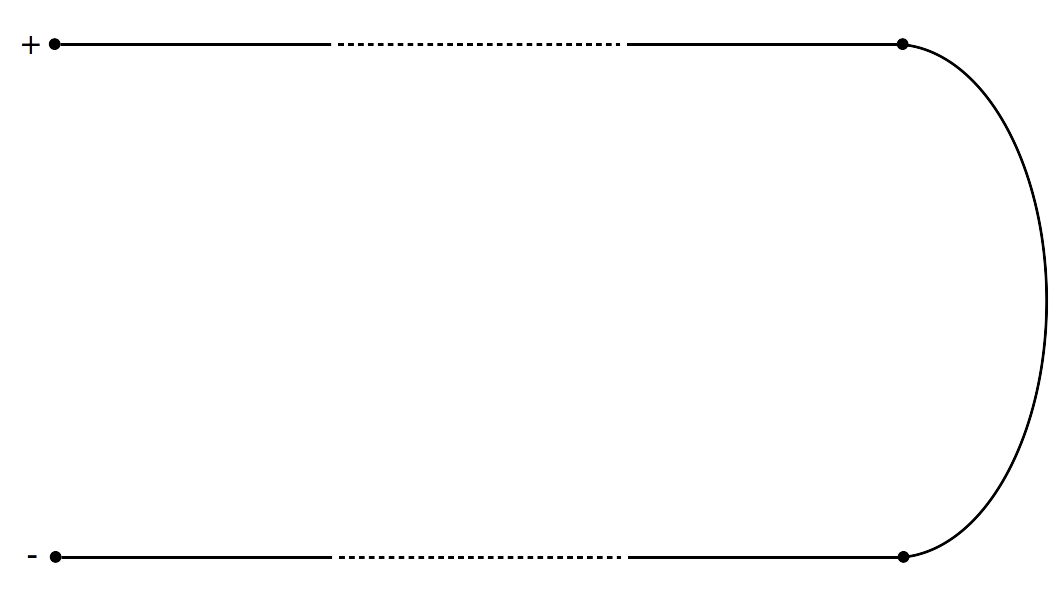
\includegraphics[width=.4\textwidth]{pictures/linea1.png}
	\label{fig:largenenough}
	\caption{\label{lul} \small Linea infinita generica}
\end{figure}

Cosa ovviamente impossibile, essendo giocoforza presenti effetti dissipativi e induttivi lungo la linea in se ed effetti capacitivi lungo il percorso, avendo noi di fatto creato un condensatore. 

La linea può essere quindi schematizzata a componenti concentrate tramite una sequenza di celle elementari composte da impedenze come
\begin{figure}[!htb]
	\centering
	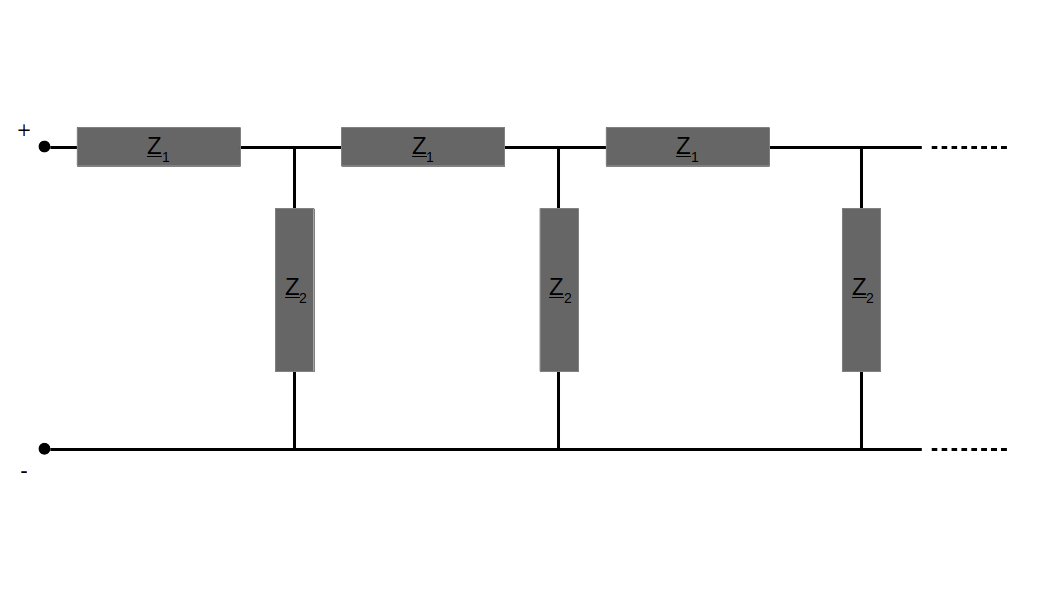
\includegraphics[width=.5\textwidth]{pictures/linea2.png}
	\label{fig:largenenough}
	\caption{\label{kekw} \small Schematizzazione della linea infinita generica}
\end{figure}

La cella elementare può essere espressa come
\begin{figure}[!htb]
	\centering
	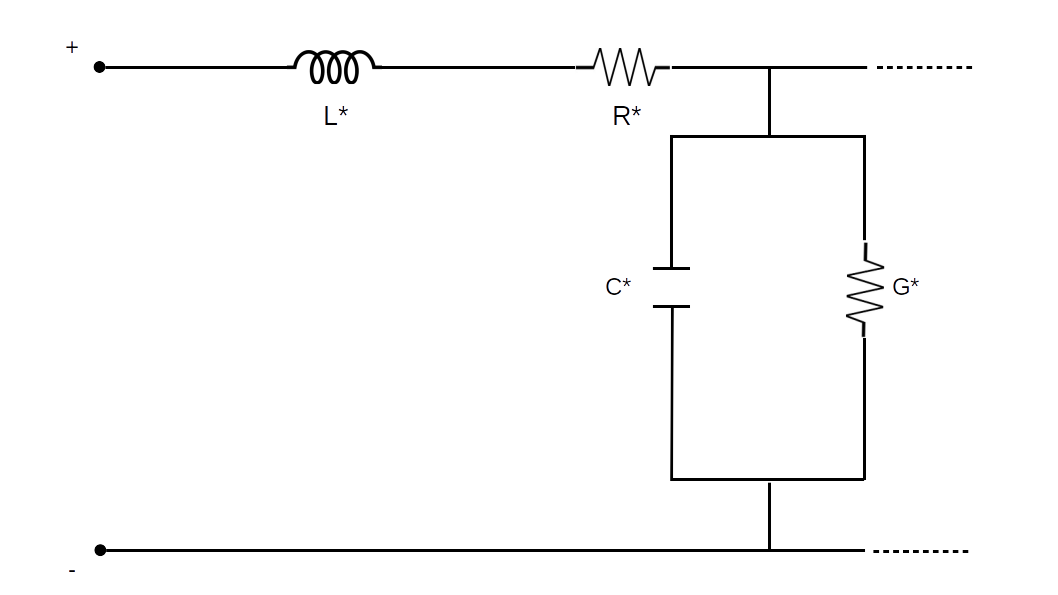
\includegraphics[width=.3\textwidth]{pictures/linea6.png}
	\label{ergwg}
	\caption{\label{luegregegl} \small Cella elementare}
\end{figure}
Dove avremo
\begin{enumerate}
	\item $L^* = L \cdot \Delta x$ Induttanza per unità di lunghezza
	\item $R^* = R \cdot \Delta x$ Resistenza per unità di lunghezza
	\item $C^* = C \cdot \Delta x$ Conduttanza per unità di lunghezza
	\item $G^* = G \cdot \Delta x$ Ammettenza per unità di lunghezza
\end{enumerate}

\newpage

Procedendo per approssimazioni, la linea può essere schematizzata come una singola impedenza
\begin{figure}[!htb]
	\centering
	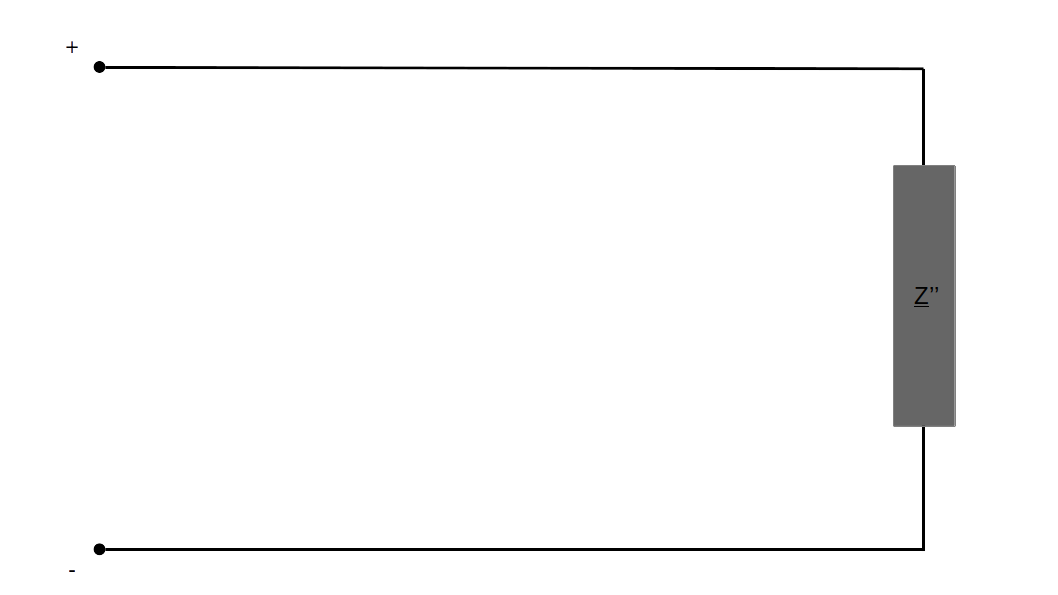
\includegraphics[width=.2\textwidth]{pictures/linea4.png}
	\label{fig:largenenough}
	\caption{\label{kekw} \small Seconda approssimazione}
\end{figure}

Il cui valore, dopo opportune approssimazioni e prendendo per assunto che le componenti passive $R$ e $G$ delle impedenze siano trascurabili, può essere stimato come
\begin{align}
Z_0 = \sqrt{\frac{L}{C}}
\end{align}

$Z_0$ prende il nome di \textbf{impedenza caratteristica} della linea infinita. Notiamo come una linea infinita si comporta come una componente interamente passiva, essendo $Z_0$ reale.


\subsection{Linea finita}

Ovviamente nella realtà non esistono linee infinite. Si avranno componenti schematizzabili come quadrupoli che fanno da tramite tra il segnale originale e un'impedenza di carico $Z_L$
\begin{figure}[!htb]
	\centering
	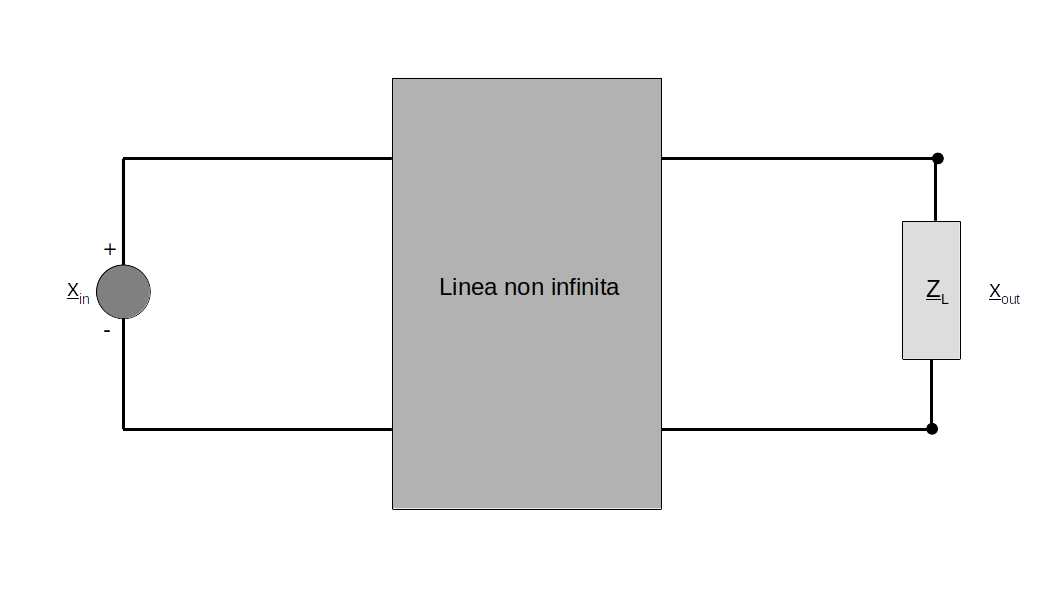
\includegraphics[width=.4\textwidth]{pictures/linea7.png}
	\label{ergwg}
	\caption{\label{luegregegl} \small Linea non infinita}
\end{figure}

Siccome abbiamo appurato che l'impedenza caratteristica è reale, ci riferiremo a entrambe come resistenze, con i nomi $R_0$ e $R_L$.

Qualora $R_L$ sia uguale a $R_0$ il generatore del segnale originario vedrà la linea come se fosse infinita, e ci sarà quin di una trasmissione completa del segnale. Si avranno altrimenti fenomeni di rilessione del segnale. Possiamo descriverli tramite il coefficiente di riflessione
\begin{align}
\rho = \frac{R_L - R_0}{R_L + R_0} \spacer \rho \in [-1 ,+1]
\end{align} 

Ci si presentano quindi tre scenari
\begin{enumerate}
	\item $R_L =R_0 \spacer \rho = 0$
	
	Si parla qui di adattamento in potenza della linea, dove il segnale viene trasmesso nella sua interezza. Si avrà di solito un dimezzamento dell'ampiezza dovuto ad effetti di partizione con la resistenza parassita del generatore.
	
	\item $R_L > R_0 \spacer \rho \in (0,+1]$
	
	Si ha in questo caso un fenomeno di interferenza costruttiva, che porta ad un'amplificazione del segnale in uscita.
	
	\item $R_L < R_0 \spacer \rho \in [-1,0)$

	Si ha in questo caso un fenomeno di interferenza distruttiva, che porta ad un'attenuazione del segnale in uscita.	
\end{enumerate}

\newpage

\subsection{Velocità di trasmissione e costante dielettrica}
La linea di trasmissione utilizzata in laboratorio è un cavo coassiale, schematizzabile in sezione come
\begin{figure}[!htb]
	\centering
	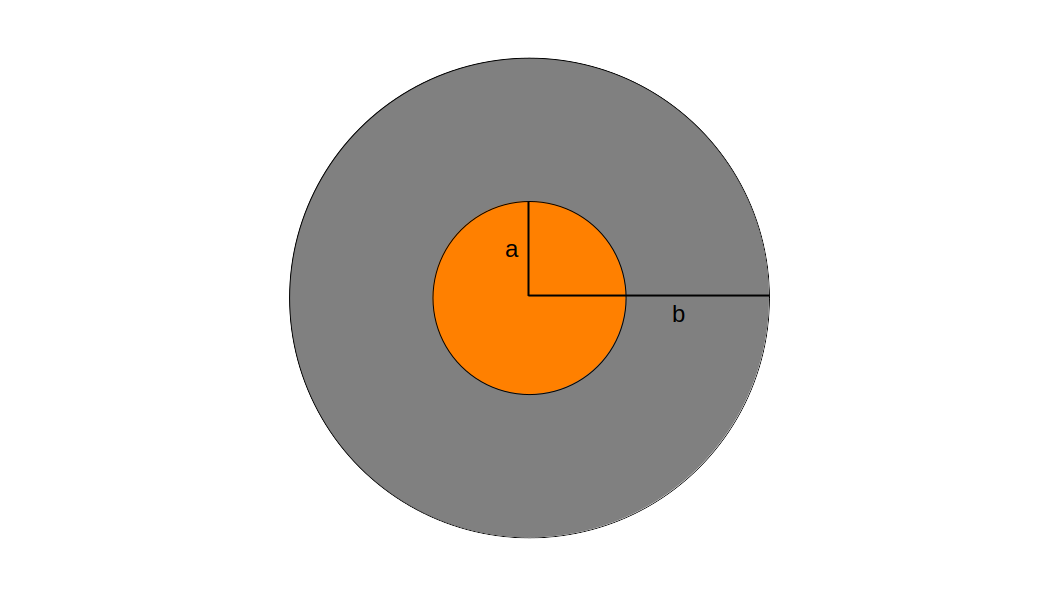
\includegraphics[width=.7\textwidth]{pictures/cavo.png}
	\label{ergwg}
	\caption{\label{luegregegl} \small Sezione del cavo}
\end{figure}


I cui parametri distribuiti sono esprimibili come
\begin{align}
&L^* = \frac{\mu}{2\pi}\cdot \ln \left(\frac{b}{a}\right)\\
&C^* = \frac{2\pi \epsilon}{\ln \left(\frac{b}{a}\right)}
\end{align}

Ricordando come
\begin{align}
&\mu = \mu_0 \cdot \mu_r\\
&\epsilon = \epsilon_0 \cdot \epsilon_r\\
&c= \frac{1}{\sqrt{\mu_0 \cdot \epsilon_0}}
\end{align}

E ponendo l'ipotesi $\mu_r=1$ (nei casi oggetto dei nostri studi molto cosistenti) otteniamo
\begin{align}
v = \frac{1}{\sqrt{\mu \cdot \epsilon}} \simeq c \cdot \frac{1}{\sqrt{\epsilon_r}} \rightarrow \epsilon_r \sim \left(\frac{c}{v} \right)^2
\end{align}

\newpage

\section{Attività sperimentale}

Per l'esperienza si è utilizzata una linea di lunghezza $l= 18 \; m$ e impedenza caratteristica di $R_0= 50 \; \Omega$.

Sfortunatamente non sono disponibili i dati presi con l'oscilloscopio in base ai quali si sono fatti i calcoli, al momento bloccati nel pc del laboratorio.

\subsection{Calcolo del coefficiente dielettrico della linea}

Questa parte riguarda le misure che si è riusciti a prendere in laboratorio.

Come prima cosa si è calcolato il tempo di viaggio del segnale, mettendo un carico molto grande e vedendo sull'oscilloscopio dopo quanto si aveva interferenza costruttiva, dividendo quel tempo per due. Si è così ottenuto
\begin{align}
t_c = 89 \; ns = 8.9 \cdot 10^{-8} \; s
\end{align}

Questo ci permette di calcolare la velocità del segnale nella linea come
\begin{align}
v = \frac{l}{t_c} = \frac{18}{8.9} \cdot  10^{8} \; \frac{m}{s} \simeq 0.2 \cdot 10^{8} \; \frac{[m]}{[s]} = 2 \cdot 10^5 \; \frac{[km]}{[s]}
\end{align}

Sapendo che $c = 3 \cdot 10^5 \; \frac{[km]}{[s]}$ abbiamo quindi ricavato
\begin{align}
\epsilon_r \simeq \left(\frac{c}{v}\right) ^2 = 2.25
\end{align}

Ci troviamo quindi in presenza di un cavo di polietilene.

\subsection{Stima dei parametri della linea}

Vista l'impossibilità di proseguire le misure in laboratorio, si è pensato di simulare la linea su SIMetrix, utilizzando una Lossy Transmission Line (RLGC).

Ci si è dunque presentata la sfida di calcolare i valori dei 4 parametri da inserire.

Per nostra fortuna ci siamo trovati con tutti gli sturmenti necessari per ricavarli, seppur facendo pesanti approssimazioni, ottenendo risultati simili a quelli del laboratorio.

Iniziamo dicendo che la linea in laboratorio presentava un comportamento quasi ideale, rumore permettendo, e si è quindi deciso di porre il più piccoli possibile i valori della reistenza e dell'ammettenza parassite, ovvero
\begin{align}
&R = 1 \; [n\Omega]\\
&G = 1 \; [nS]
\end{align}

Il problema si è dunque ridotto al calcolo di $L$ e di $C$. 
Dall'espressione dell'impedenza caratteristica si ricava che
\begin{align}
L= R_0^2\cdot C  \; [H]\label{lmaoao}
\end{align}

Da quanto detto nelle scorse pagine sappiamo anche la velocità del segnale nella linea è data da
\begin{align}
v = \frac{1}{\sqrt{L^*C^*}} \; \frac{[m]}{[s]}
\end{align}

Siccome possiamo esprimere i parametri distribuiti come
\begin{align}
L^* = \frac{L}{\Delta x}  \; \frac{[H]}{[m]}
\end{align}

Facendo la pesante approssimazione di porre $|\Delta x|=1$ otteniamo
\begin{align}
v = \frac{1}{\sqrt{LC}} \label{cdfdf}  \; \frac{[m]}{[s]}
\end{align}

Inserendo la \ref{lmaoao} nella \ref{cdfdf} otteniamo
\begin{align}
&v = \frac{1}{R_0 C} \; \frac{[m]}{[s]} \firstpassage
&C = \frac{1}{R_0 v} \; [F]
\end{align}

Avendo calcolato la velocità del segnale nel paragrafo precedente ed essendo nota l'impedenza caratteristica della nostra linea, possiamo dunque ricavare entrambe le nostre incognite
\begin{align}
&C = \frac{1}{50 \cdot 2} \cdot 10^{-8} \; [F] = 100 \; [pF]\\
&L = 2500 \cdot  10^{-10} \; [H] = 250 \; [nH]
\end{align}



\section{Simulazione su SIMetrix e studio del segnale}

\subsection{Circuito simulato, segnale in ingresso e considerazioni iniziali}
In base a quanto detto finora si è progettato su SIMetrix il seguente circuito
\begin{figure}[!htb]
	\centering
	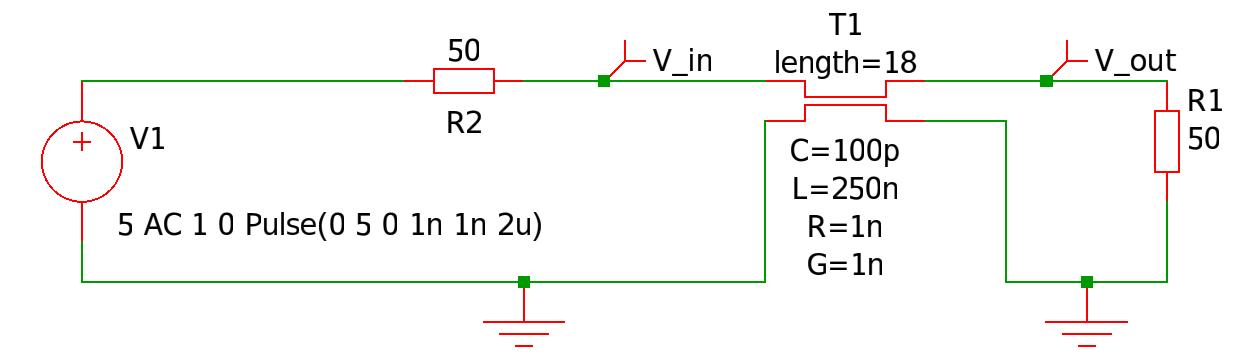
\includegraphics[width=\textwidth]{pictures/linea.png}
	\label{ergwg}
	\caption{\label{luegregegl} \small Schematica del circuito nel caso di linea adattara}
\end{figure}

Si è scelto di simulare un generatore reale di tensione mettendo in serie al generatore ideale $V_1$ la resistenza $R_2$.

Per le misure si è scelto di mandare un impulso con le seguenti caratteristiche
\begin{enumerate}
	\item Tempo di salita e discesa pari a $1 \; [ns]$
	\item Larghezza $2 \; [\mu s]$
	\item Minimo di ampiezza $V_{min} = 0 \; [V]$
	\item Massimo di ampiezza $V_{max} = 5 \; [V]$
	\item Offset pari a  $2.5 \; [V]$
	\item Ampiezza complessiva  $\Delta V= 5 \; [V]$
\end{enumerate}

E ci si è concentrati sullo studio dei fronti di salita.

Utlizzando i valori ricavati nello scorso paragrafo, si è ottenuta una linea, come si noterà nei prossimi plot, con tempo di viaggio del sengale pari a $90 \; [ns]$, che è una stima più che buona del valore misurato in laboratorio, che era  $89 \; [ns]$


\newpage

\subsection{Presa dati}

\subsubsection{Adattamento in potenza}

Iniziamo ad esempio dalla linea adattata in potenza sul carico. Il risultato della simulazione restituisce
\begin{figure}[!htb]
	\centering
	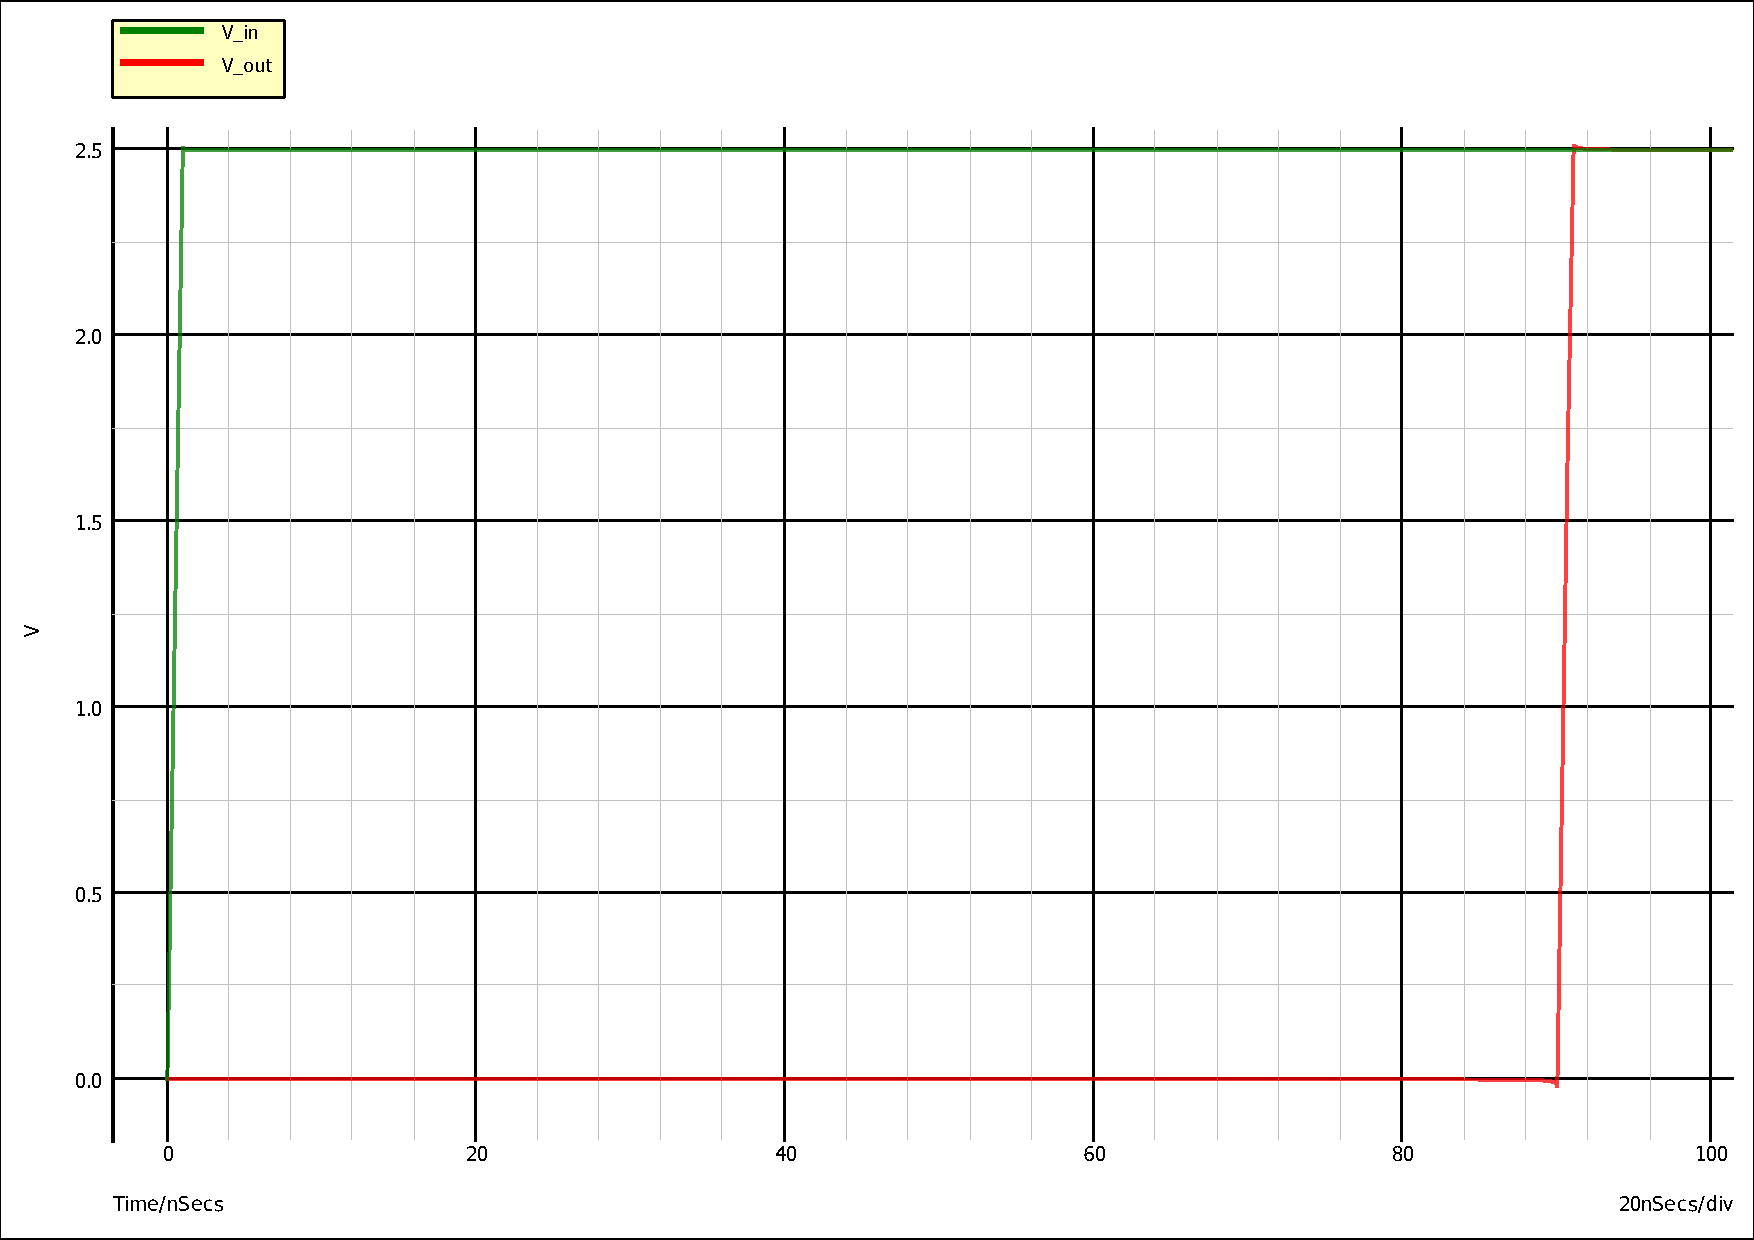
\includegraphics[width=\textwidth]{pictures/Adattamento_in_potenza.pdf}
	\label{ergwg}
	\caption{\label{luegregegl} \small Schematica del circuito nel caso di linea adattata}
\end{figure}

Notiamo come la linea si comporti esattamente come ci si aspetta dalla teoria, con un dimezzamento dell'ampiezza nominale del segnale, dovuta all'effetto di partizione fra la linea adattata e la resistenza parassita $R_2$, e un ritardo nel segnale $V_{out}$ di $90 \; [ns]$, con però ampiezza uguale a quella di $V_{in}$.


\newpage

\subsubsection{Riflessione con interferenza costruttiva}

Vediamo ora come cambia il segnale in ingresso aumentando progressivamente il valore della resistenza di carico, avvicinandoci man mano al caso limite $\rho =1$. Presentiamo di seguito i grafici per i seguenti valori del carico $R_1$: 
\begin{enumerate}
	\item $100 \; [\Omega]$	
	\item $200 \; [\Omega]$	
	\item $500 \; [\Omega]$
	\item $5 \; [k\Omega]$
	\item $5 \; [M\Omega]$
\end{enumerate}

Quello che ci si aspetta dalla teoria è una crescita del segnale in ingresso dopo $180 \; [ns]$, sempre più significativo man mano che si alza il valore del carico, ovvero il tempo di andata e ritorno del segnale dal carico. Come si può vedere dai grafici riportati l'aspettativa è stata pienamente confermata dalla simulazione.

\begin{figure}[!htb]
	\centering
	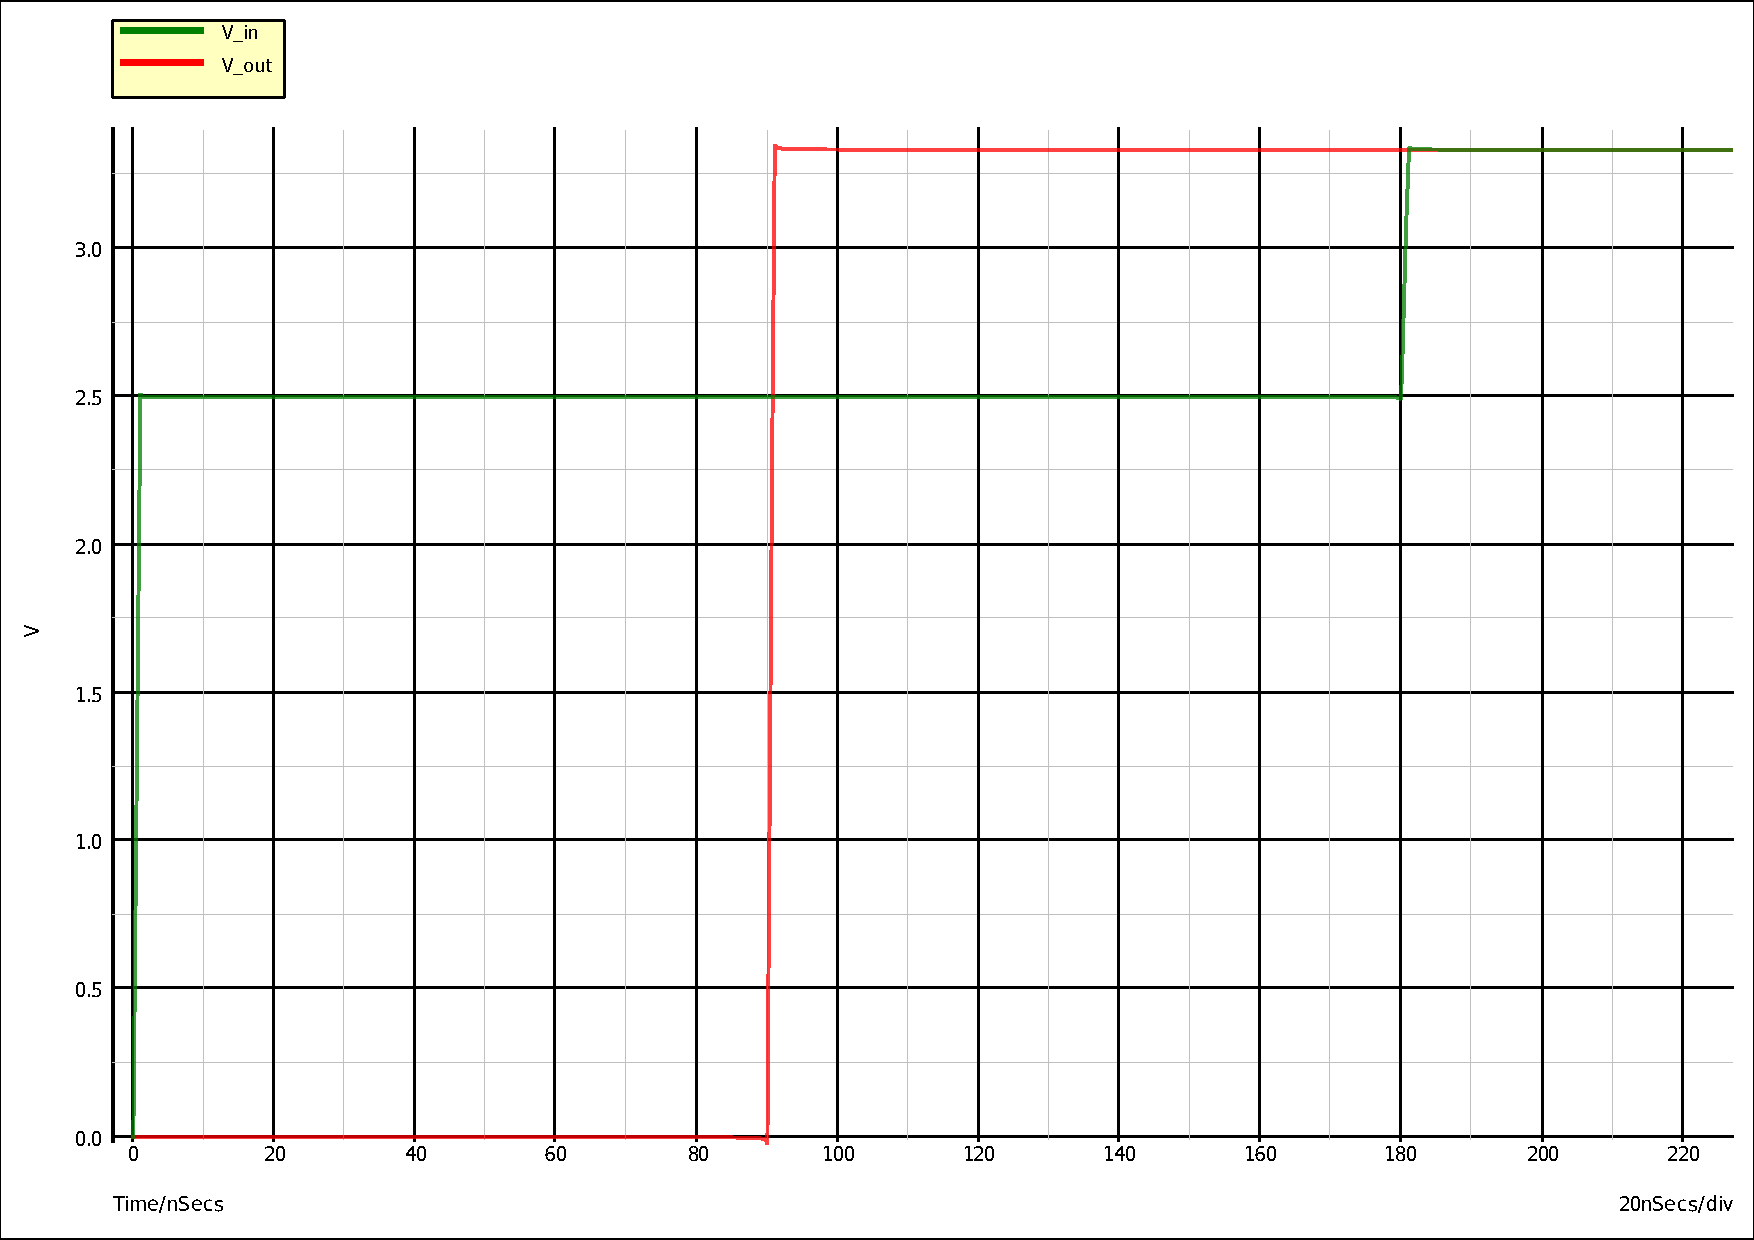
\includegraphics[width=.8\textwidth]{pictures/100ohm.pdf}
	\label{ergwxxg}
	\caption{\label{luegrevvvgegl} \small $R_1 = 100 \; [\Omega]$ }
\end{figure}

\begin{figure}[!htb]
	\centering
	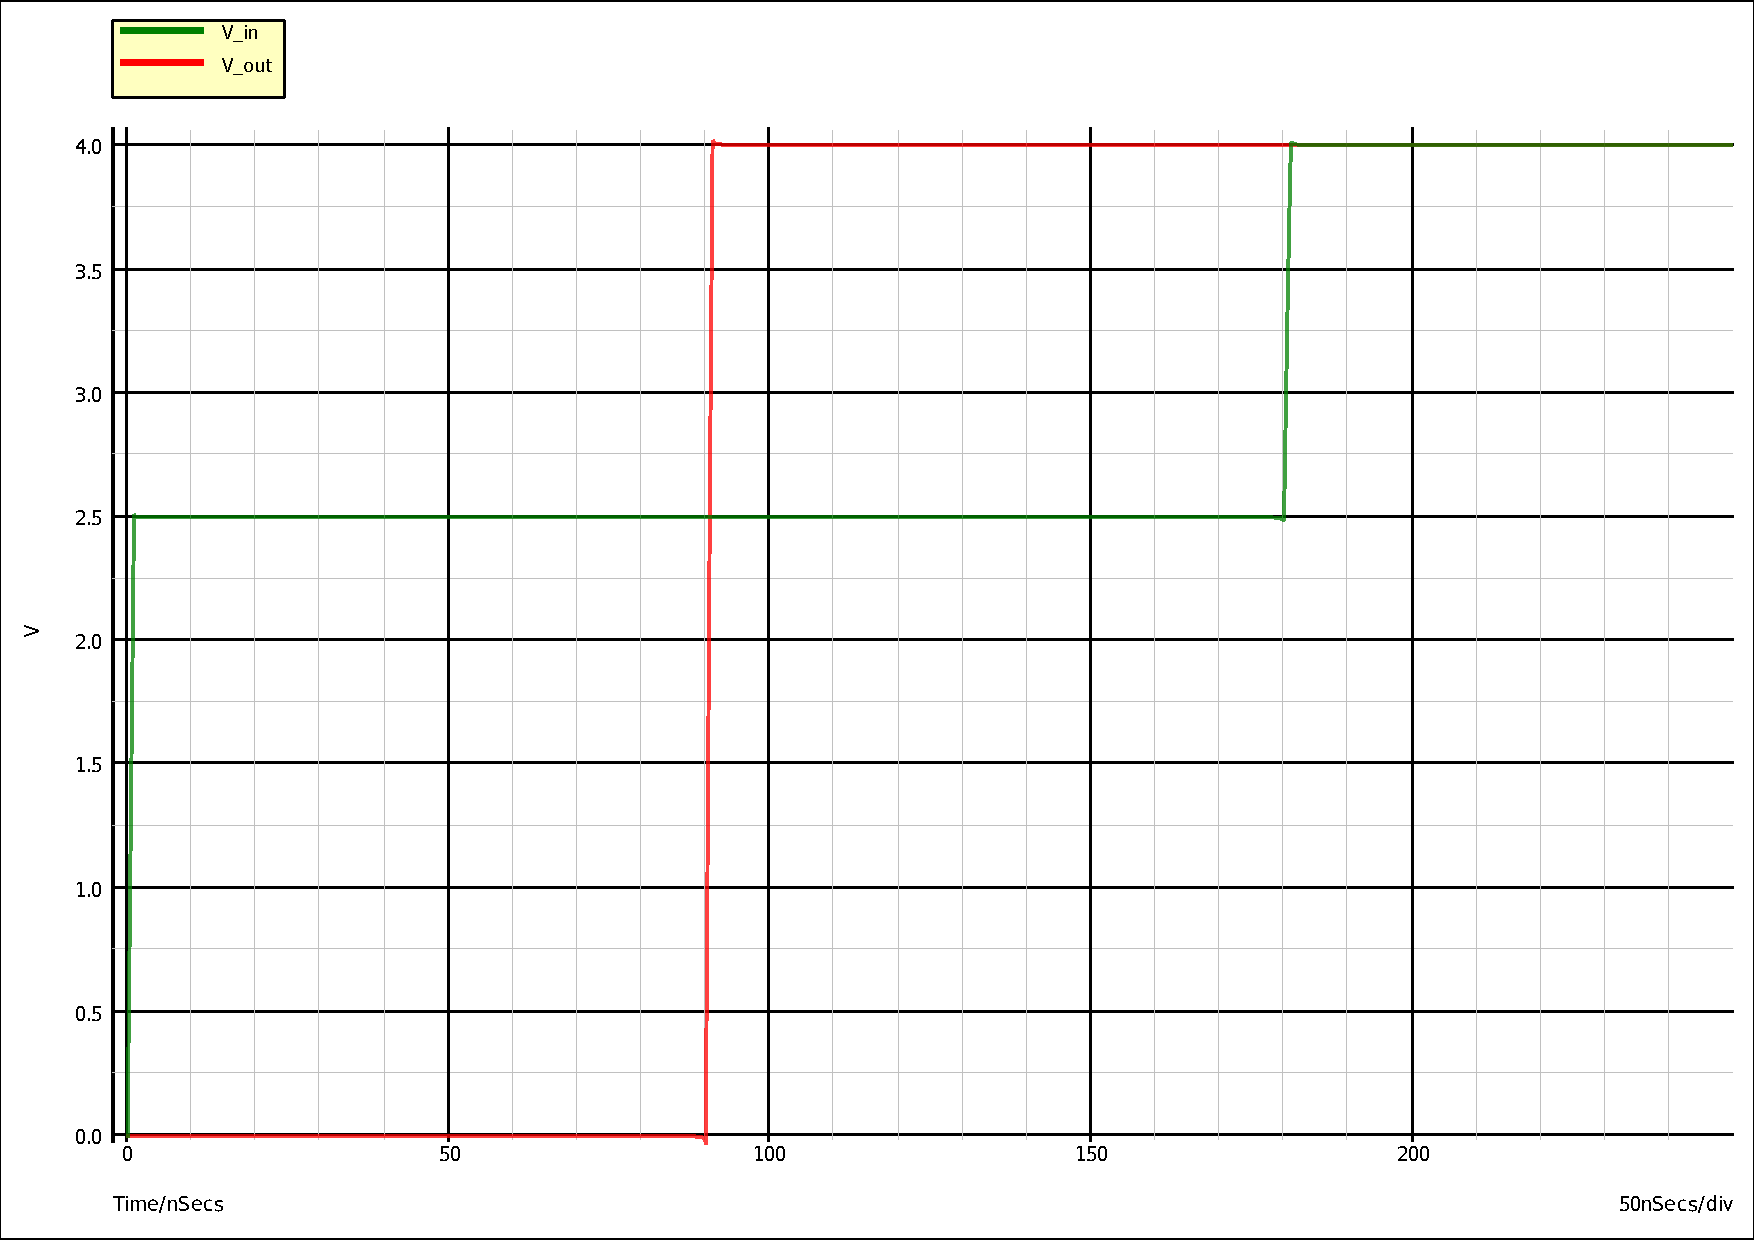
\includegraphics[width=.8\textwidth]{pictures/200ohm.pdf}
	\label{ergddwg}
	\caption{\label{luegrfffegegl} \small $R_1 = 200 \; [\Omega] $}
	\end{figure}

\begin{figure}[!htb]
	\centering
	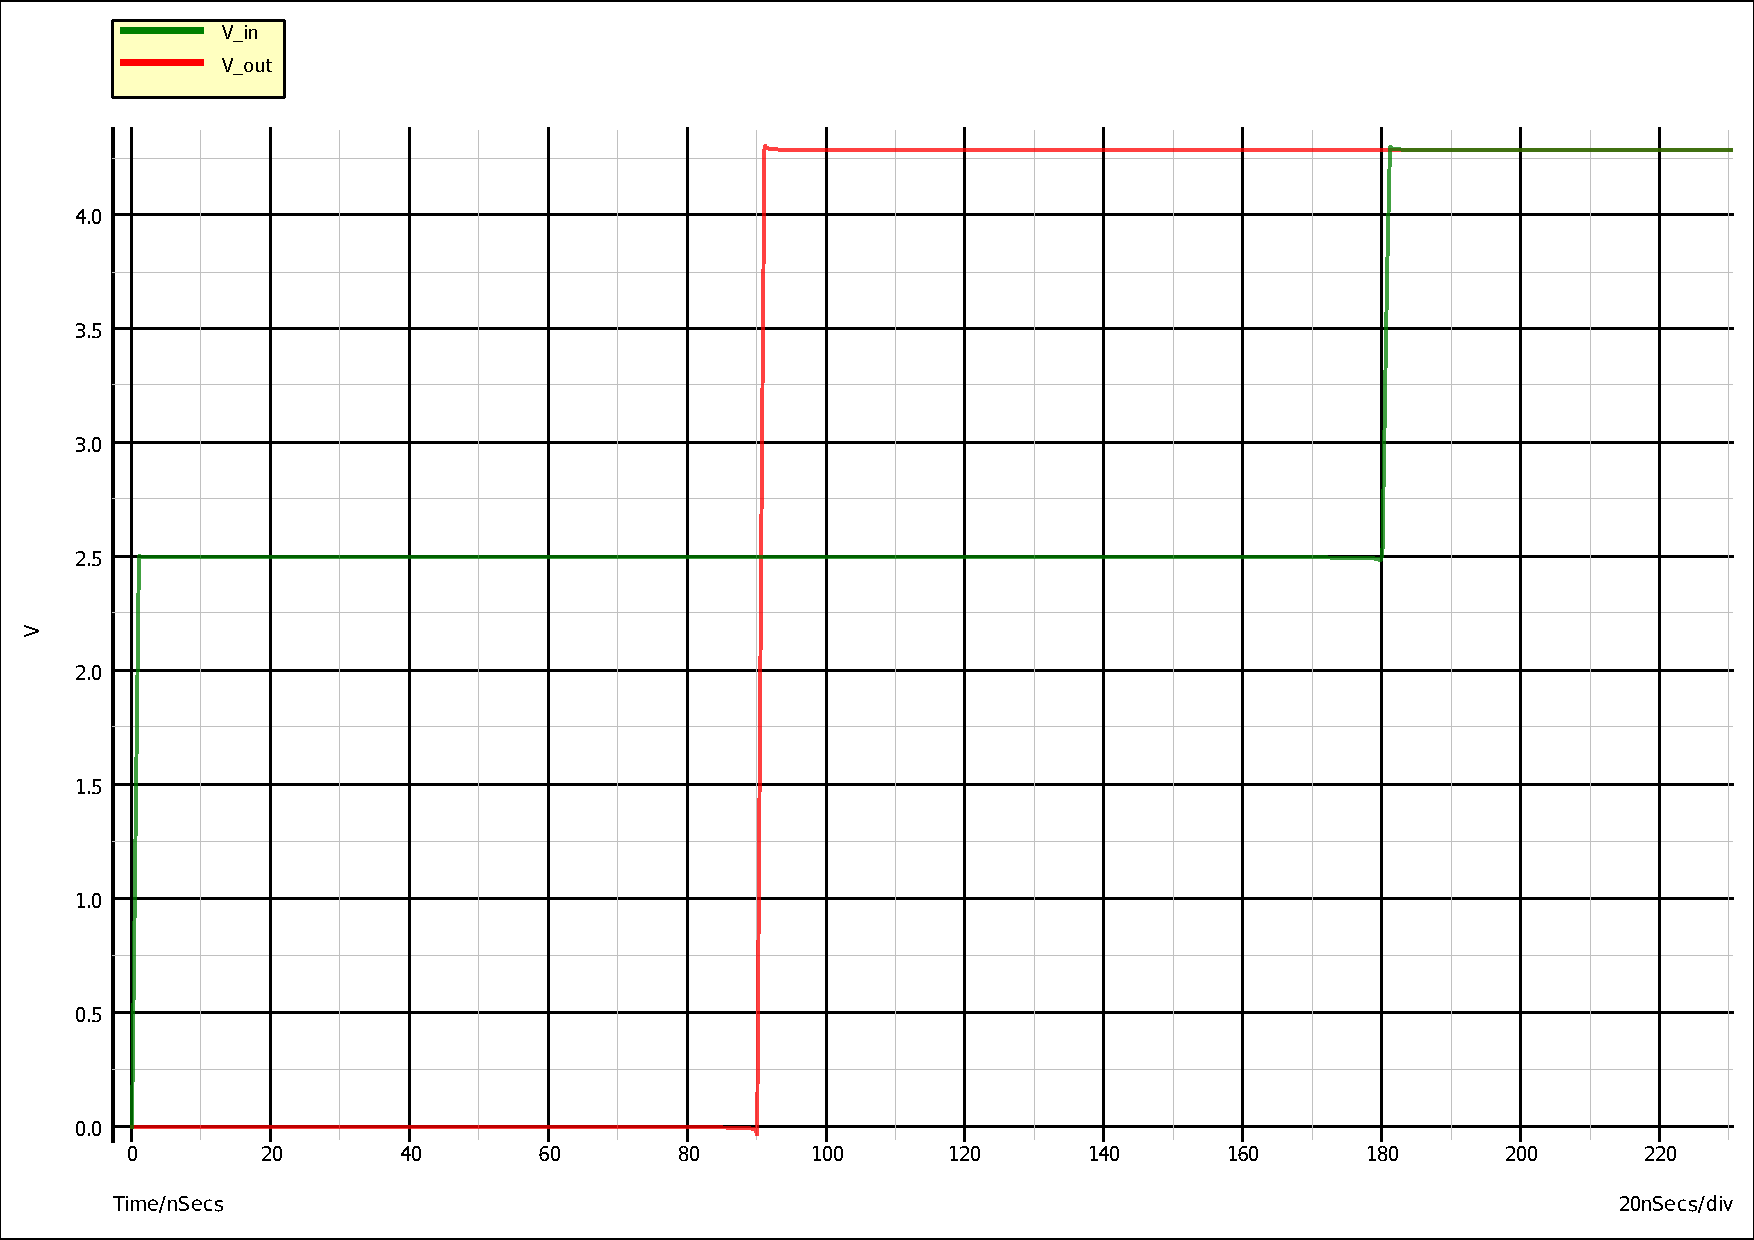
\includegraphics[width=.8\textwidth]{pictures/300ohm.pdf}
	\label{ergw33xxg}
	\caption{\label{luegr33evvvgegl} \small $R_1 = 300 \; [\Omega]$ }
\end{figure}

\begin{figure}[!htb]
	\centering
	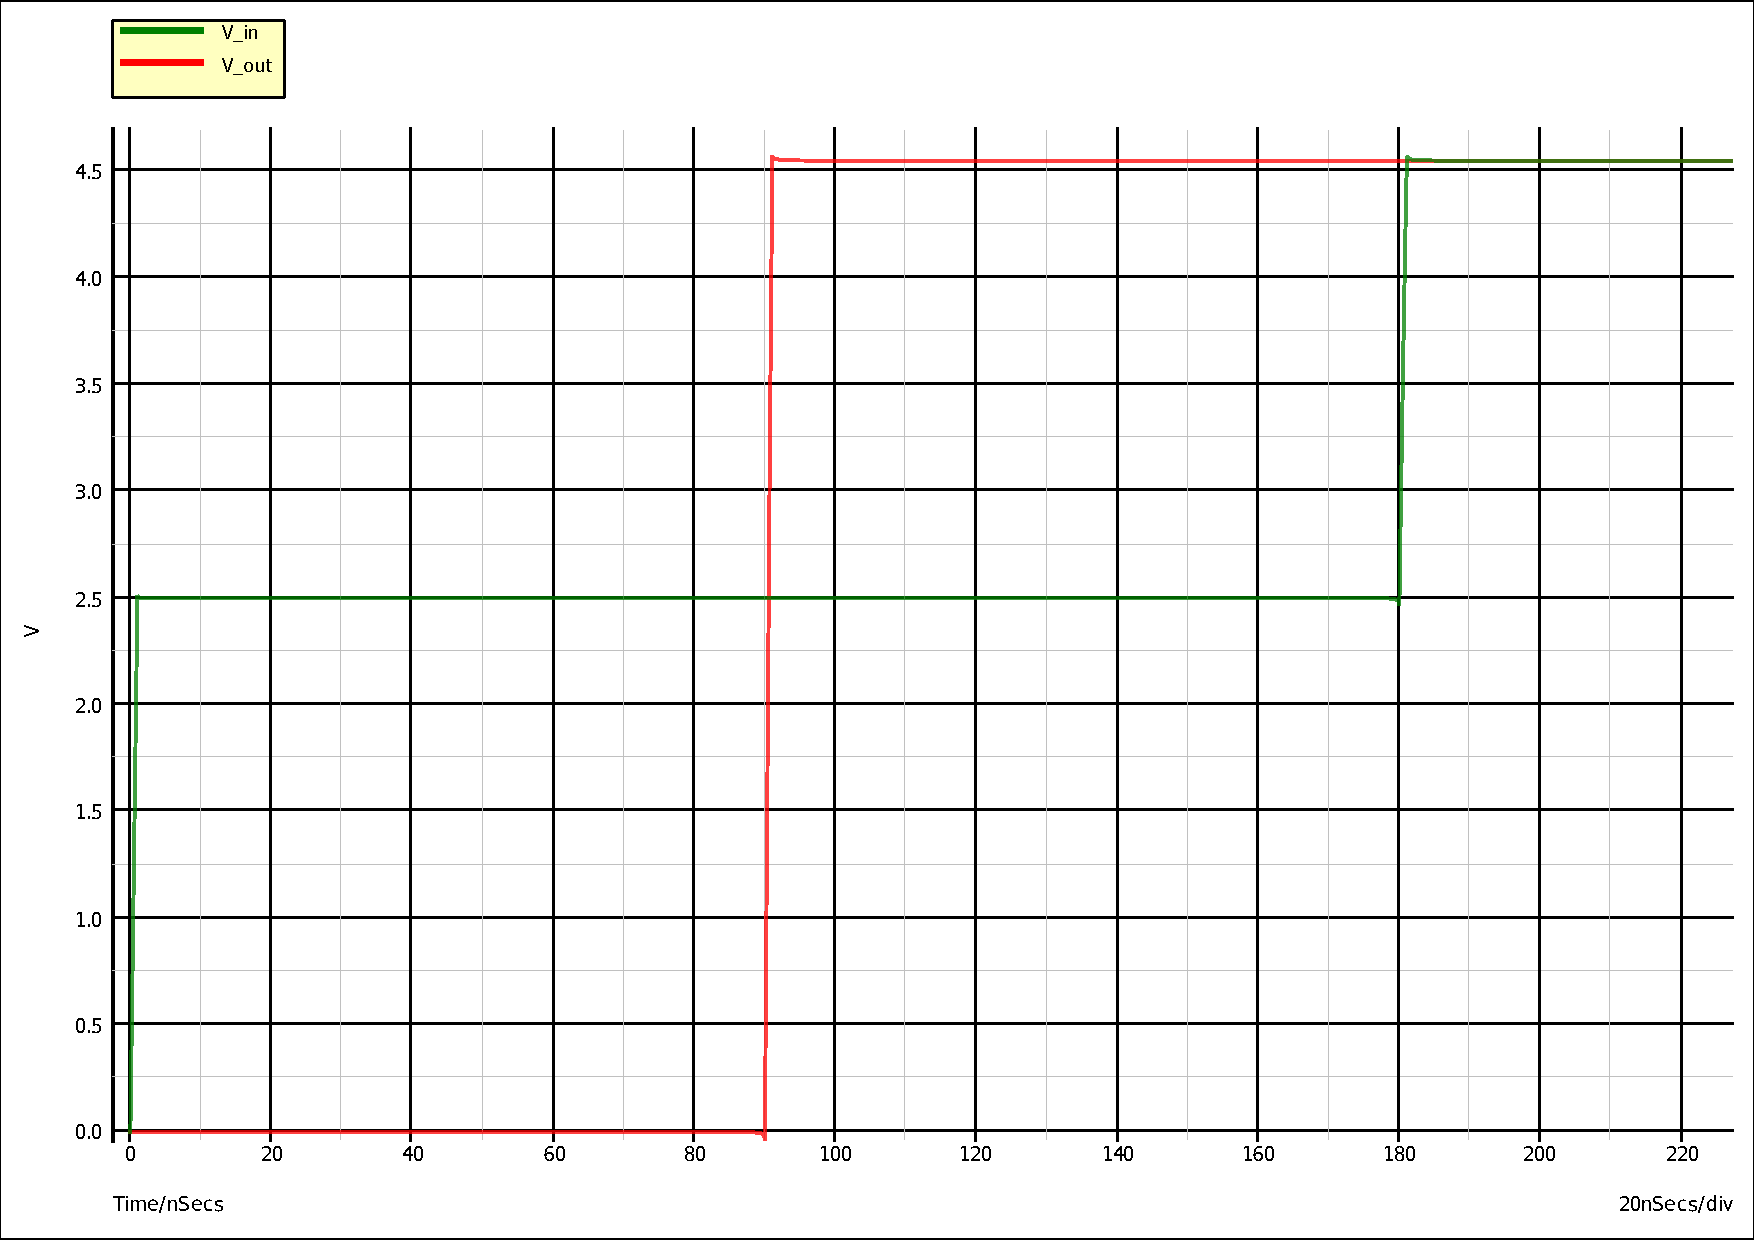
\includegraphics[width=.8\textwidth]{pictures/500ohm.pdf}
	\label{e55rgddwg}
	\caption{\label{luegr55fffegegl} \small $R_1 = 500 \; [\Omega] $}
\end{figure}

\begin{figure}[!htb]
	\centering
	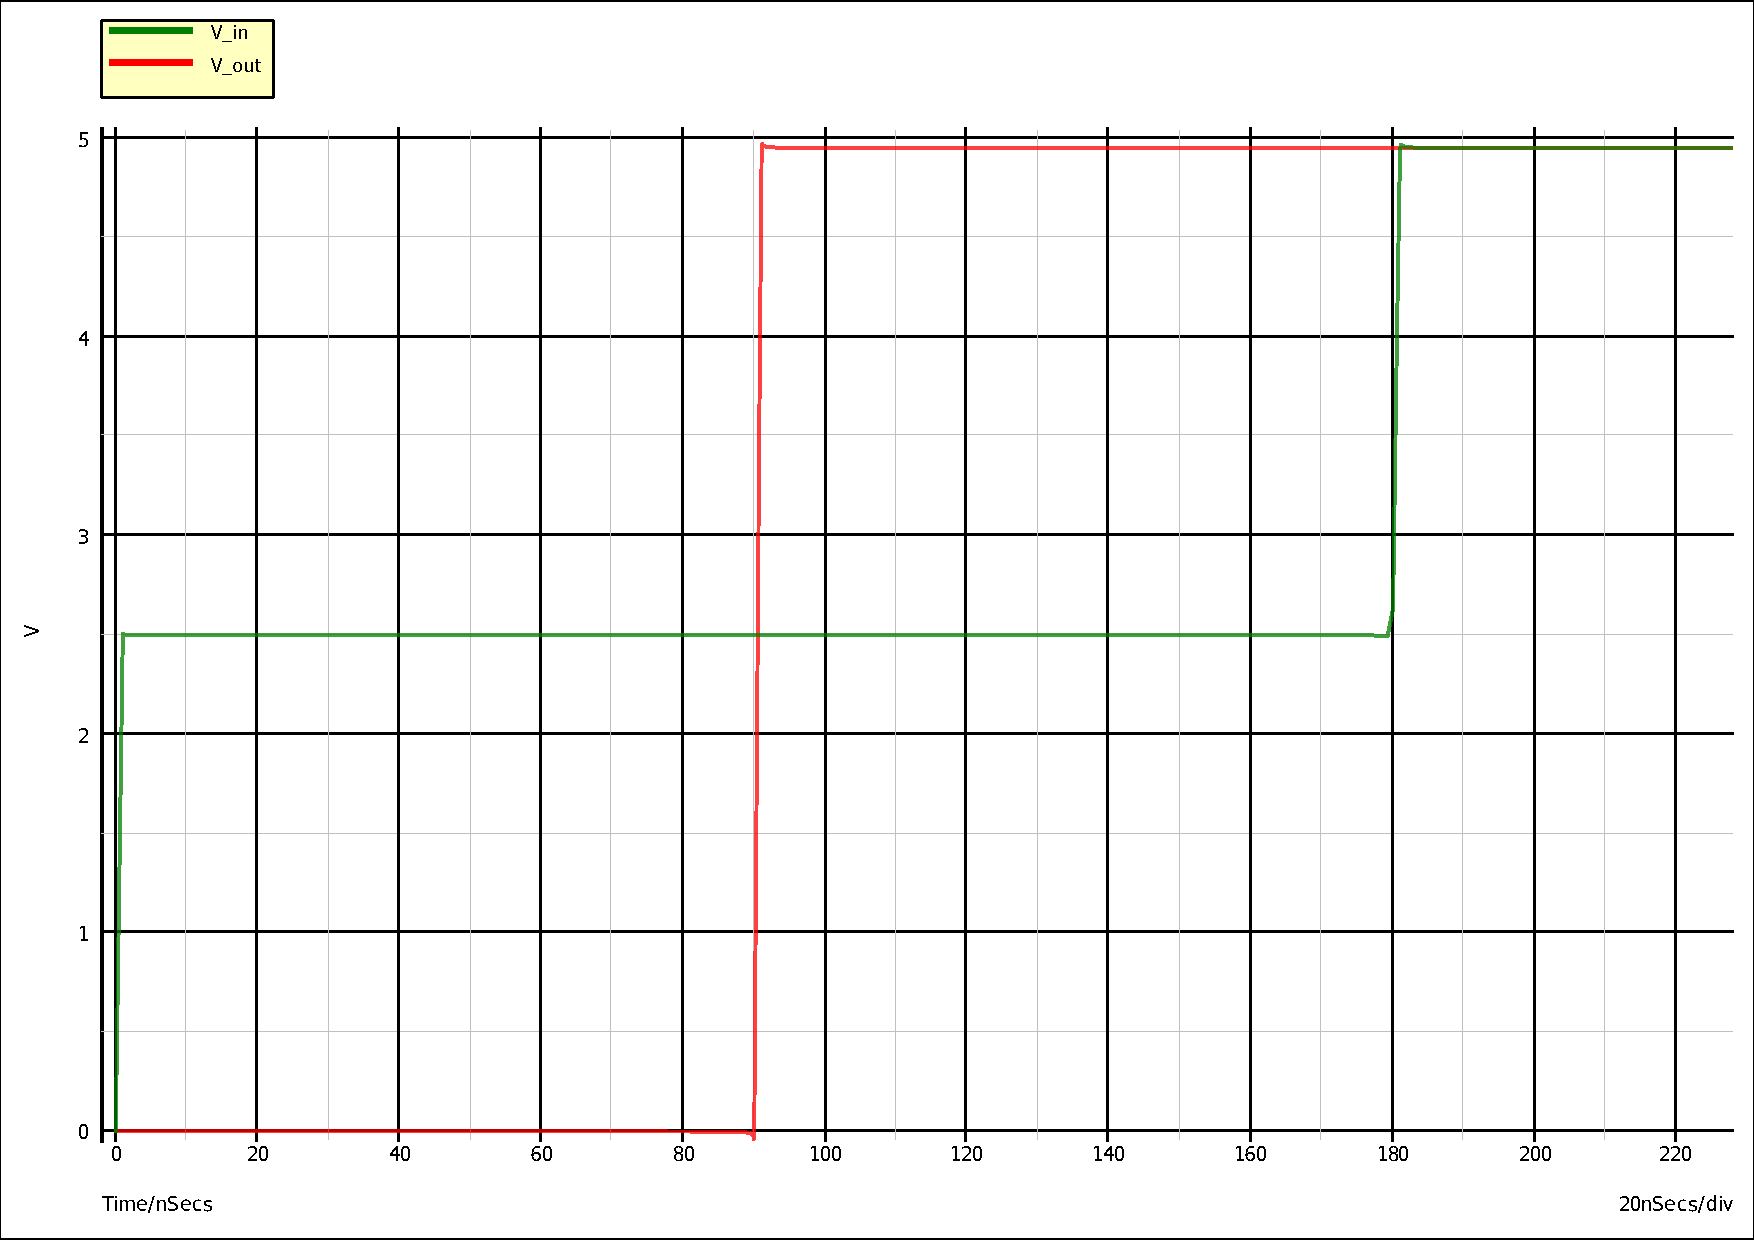
\includegraphics[width=.8\textwidth]{pictures/5kohm.pdf}
	\label{e55cccrgddwg}
	\caption{\label{luegr5ccc5fffegegl} \small $R_1 = 5 \; [k\Omega] $}
\end{figure}

\begin{figure}[!htb]
	\centering
	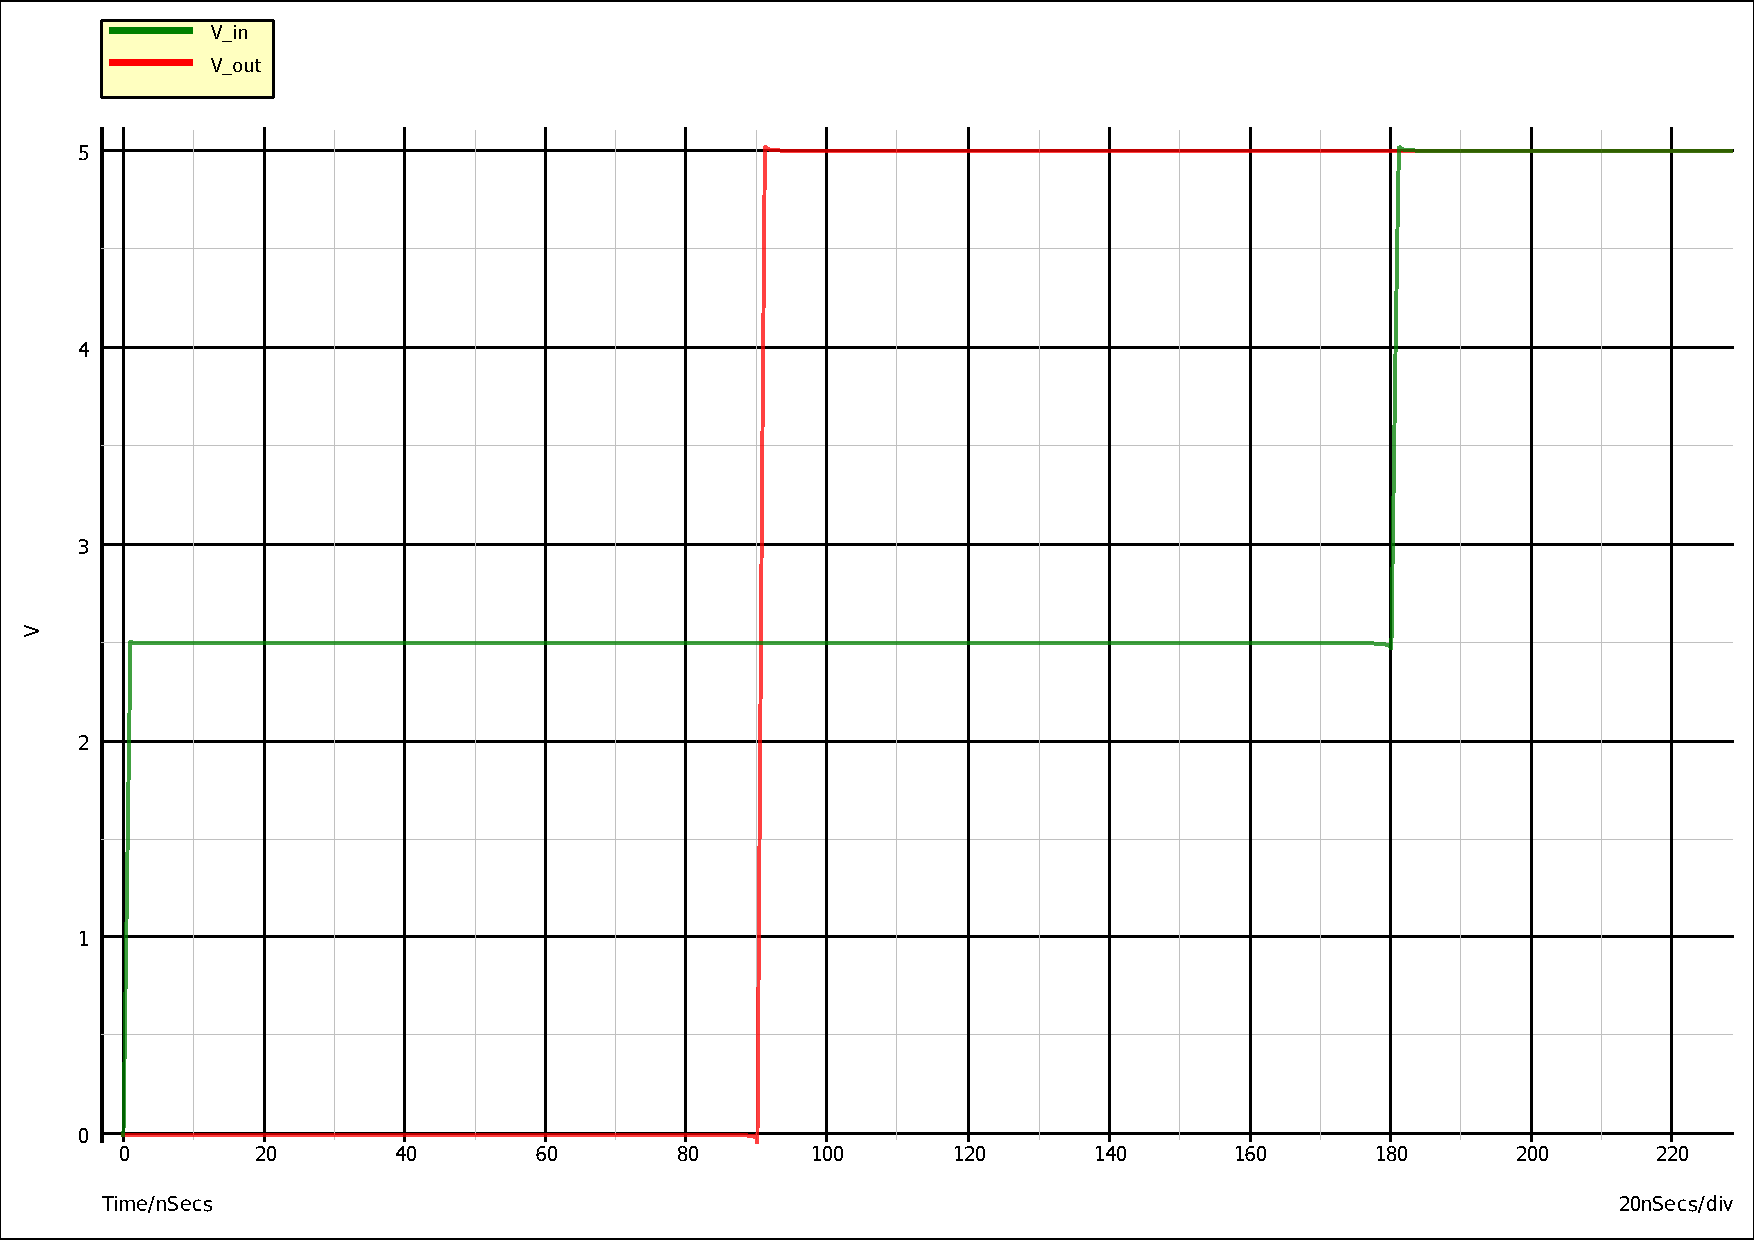
\includegraphics[width=.8\textwidth]{pictures/5Mohm.pdf}
	\label{e55rdddgddwg}
	\caption{\label{luegr55fdddffegegl} \small $R_1 = 5 \; [M\Omega] $}
\end{figure}

\clearpage

\subsubsection{Riflessione con interferenza distruttiva}

Vediamo invece cosa si ottiene abbassando il carico sotto il valore della resistenza caratteristica. Analizzeremo il risultato per i seguenti valori di $R_1$:
\begin{enumerate}
	\item $25 \; [\Omega]$	
	\item $10 \; [\Omega]$	
	\item $1 \; [\Omega]$
	\item $500 \; [m\Omega]$
	\item $50 \; [m\Omega]$
\end{enumerate}

Ci si aspetta in questo caso che, man mano che si diminuisce il valore del carico, dopo $180 \; [ns]$ il segnale venga attenuato sempre di più, sino a raggiungere quasi lo zero. 

\begin{figure}[!htb]
	\centering
	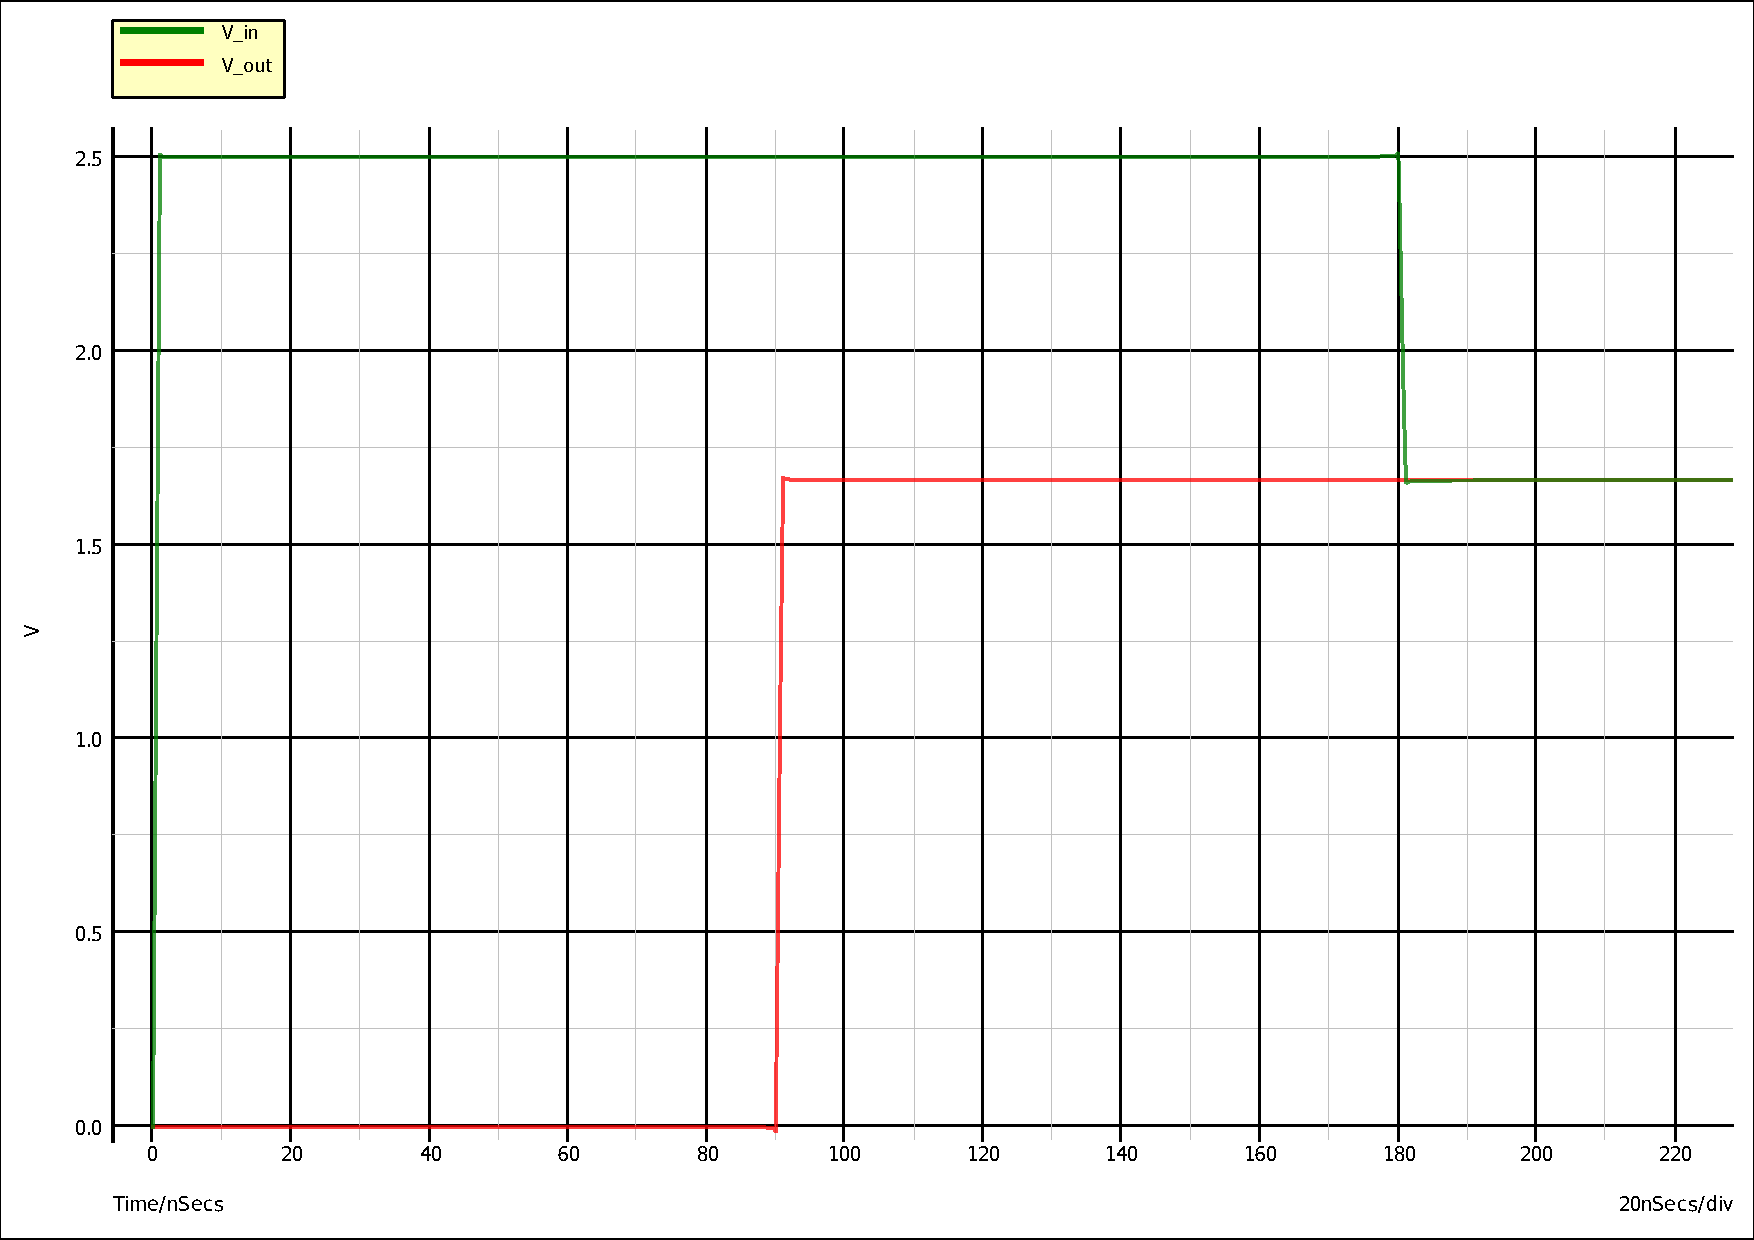
\includegraphics[width=.8\textwidth]{pictures/25ohm.pdf}
	\label{ergccwxxg}
	\caption{\label{luegreccvvvgegl} \small $R_1 = 25 \; [\Omega]$ }
\end{figure}

\begin{figure}[!htb]
	\centering
	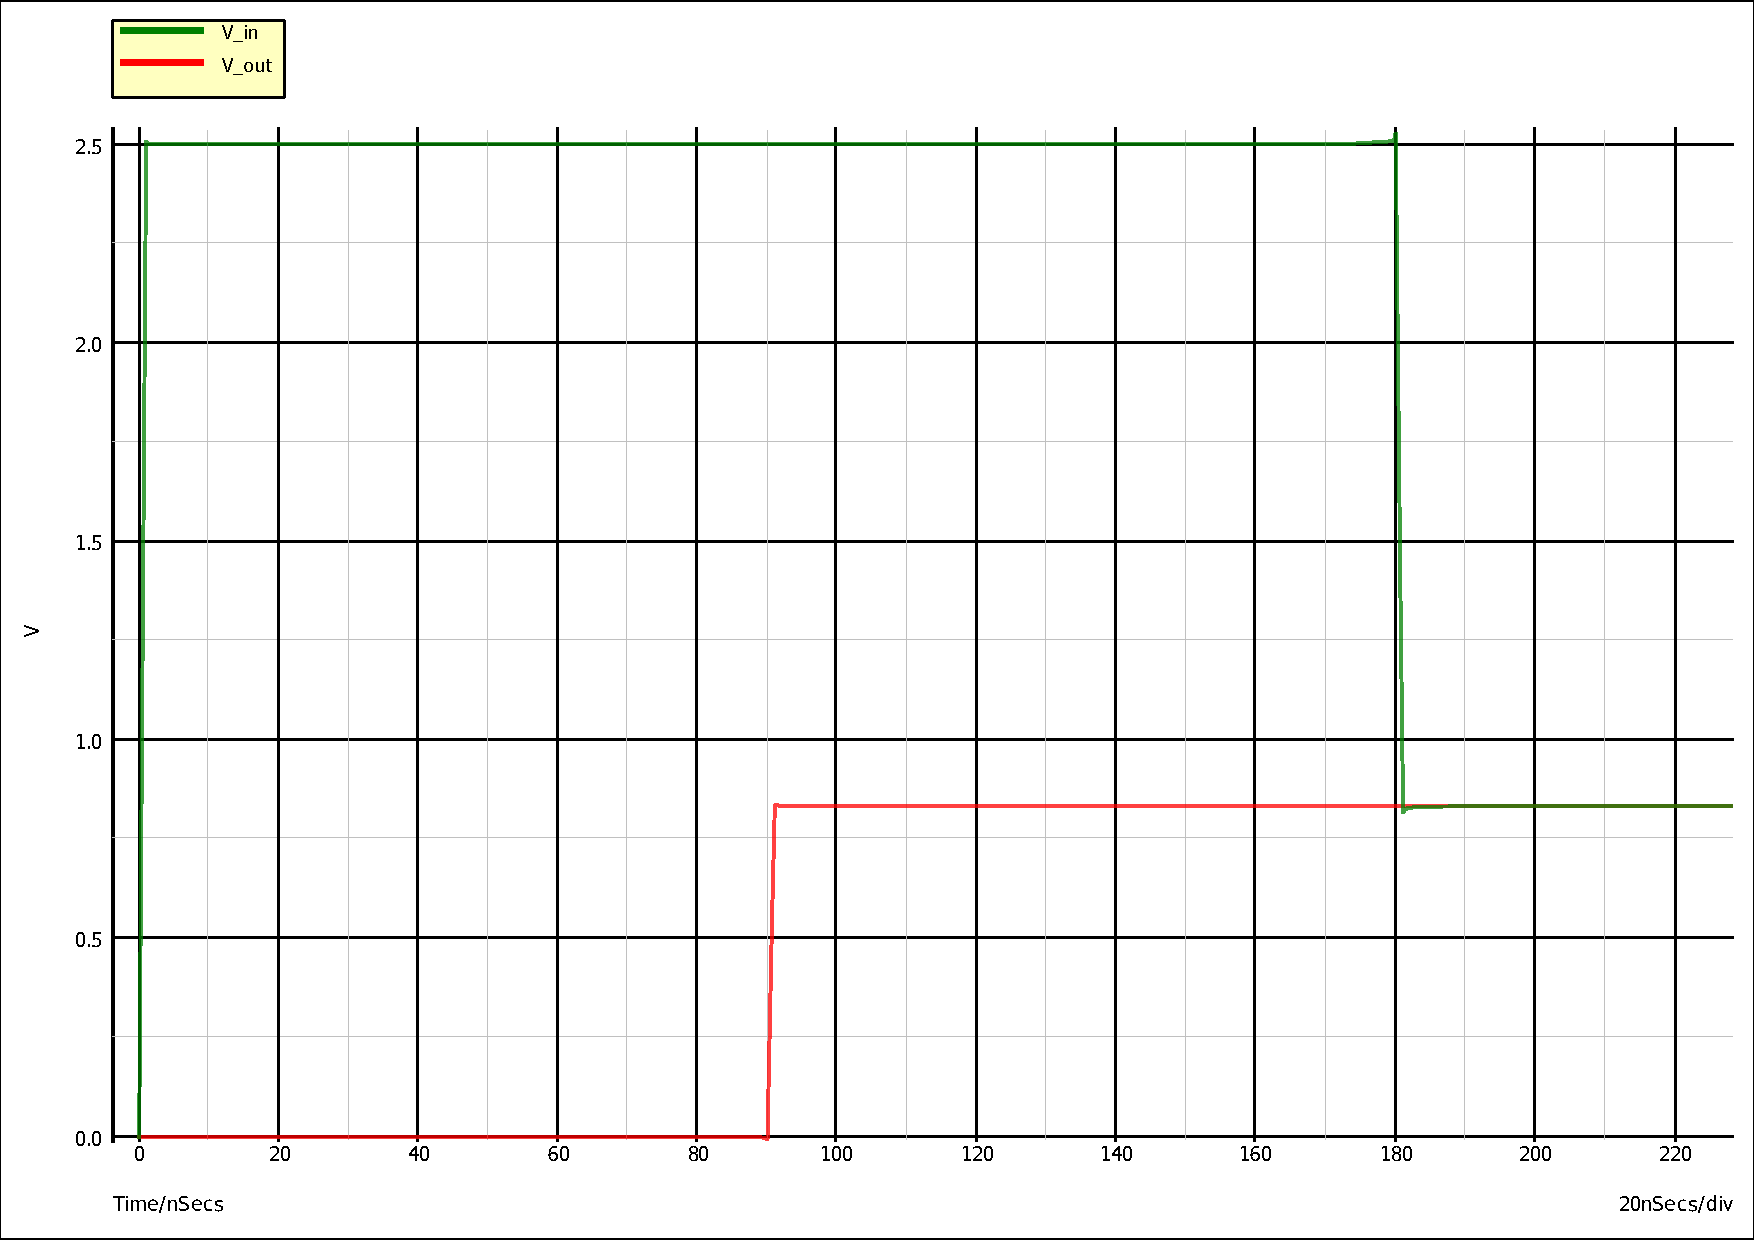
\includegraphics[width=.8\textwidth]{pictures/10ohm.pdf}
	\label{ergccwxxxxg}
	\caption{\label{luegrecczzvvvgegl} \small $R_1 = 10 \; [\Omega]$ }
\end{figure}

\begin{figure}[!htb]
	\centering
	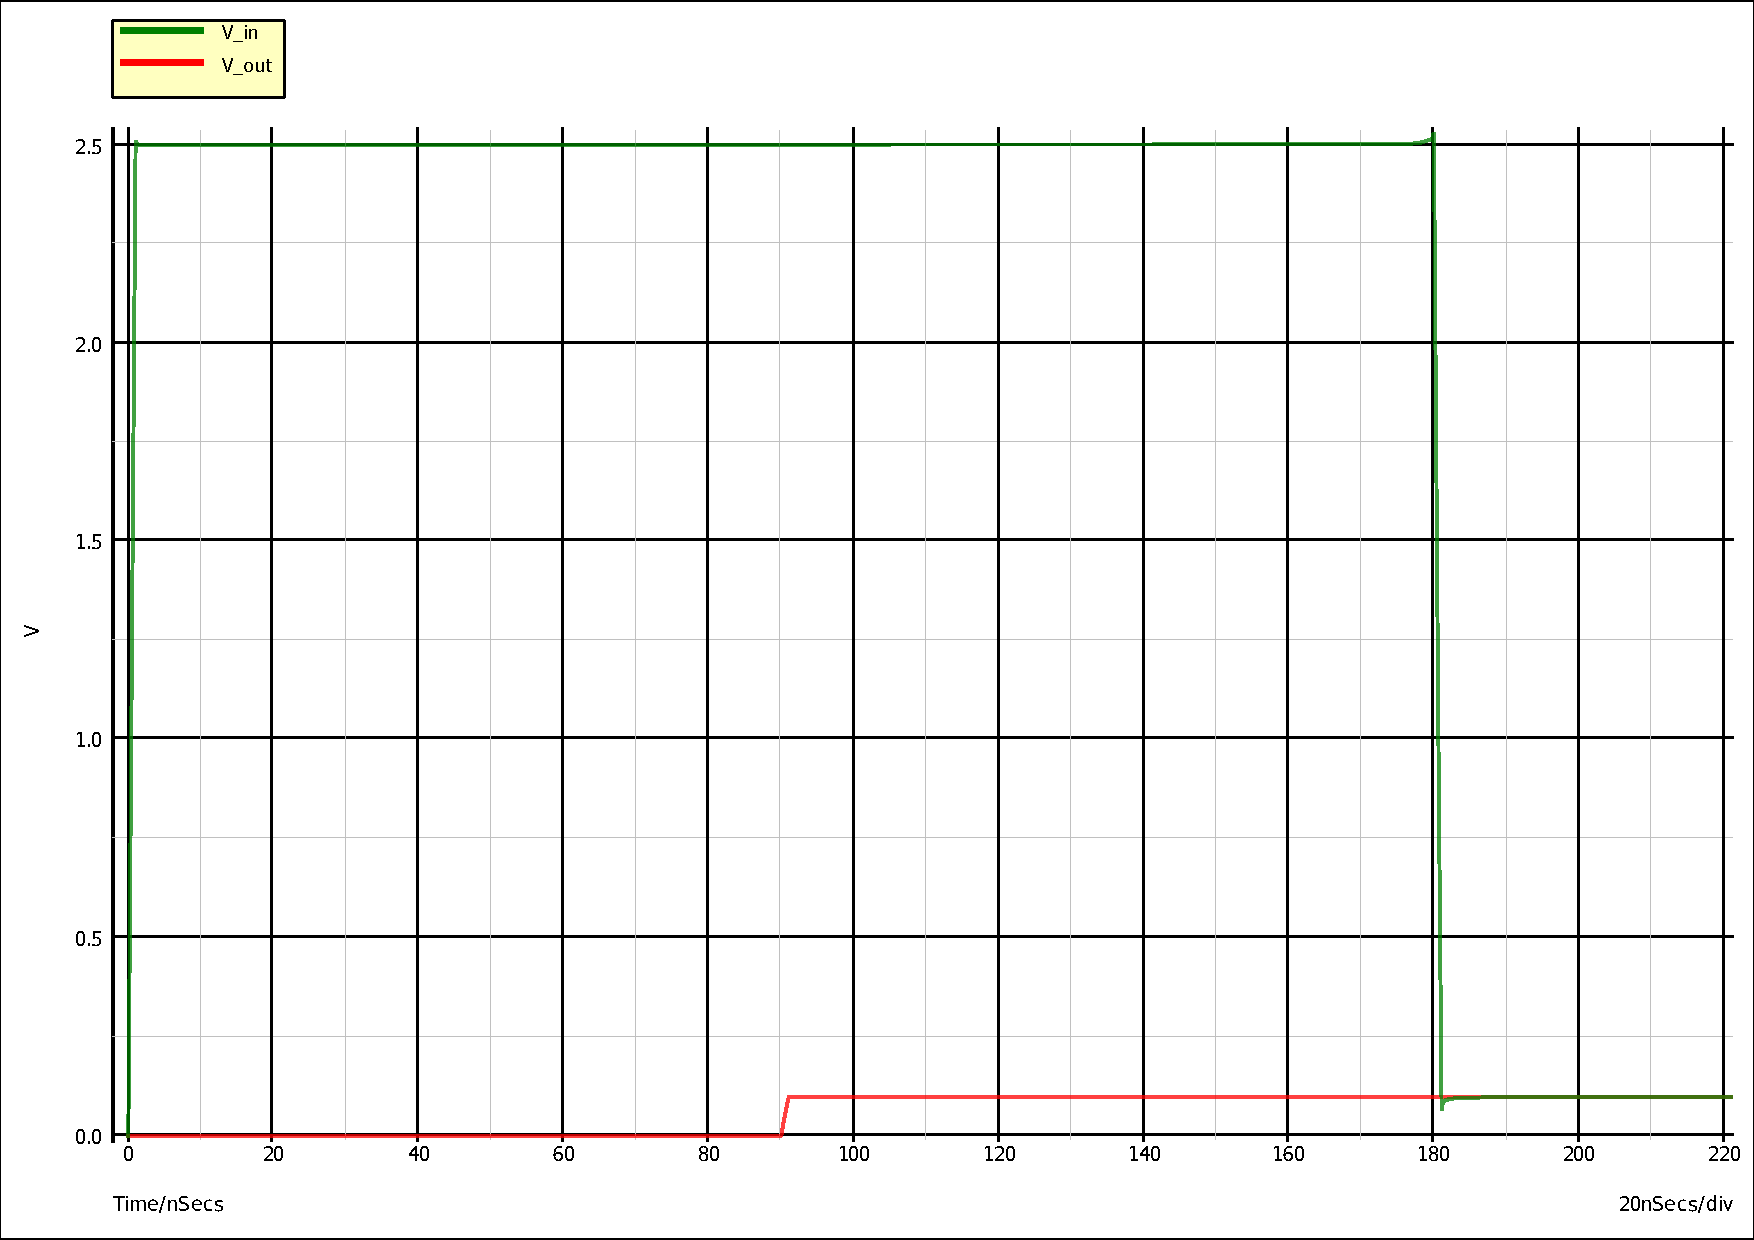
\includegraphics[width=.8\textwidth]{pictures/1ohm.pdf}
	\label{ergccwxxxxg}
	\caption{\label{luegrecczzvvvgegl} \small $R_1 = 1 \; [\Omega]$ }
\end{figure}

\end{document}